A greenhouse (also called a glasshouse) is a structure with walls and a roof made chiefly of transparent material, such as glass, in which plants requiring regulated climatic conditions are grown.\cite{greenhouse}These structures range in size from small sheds to industrial-sized buildings, according to various objects. Although greenhouse technology has shown its value in different uses, a blank still exists in the field of a home ornamental greenhouse product for ordinary consumers, especially for those people who lived in a department in an urban area. There are still several obstacles and gaps that remain to be solved for such kinds of products.

% \subsection{Background}
\subsection{Background and Problem}
Greenhouse production plays a significant role in modern agriculture, especially in densely populated areas such as eastern China. Greenhouse environmental conditions have proven efficient and essential for crop yield, pest prevention, energy saving, etc.\cite{LI2020105096} As a productive system, the large-scale and medium-scale greenhouses allows us to respond to the growing global demand for fresh and healthy crops throughout the year, which is widely applied in agricultural production.\cite{rizwan2022optimal} Traditionally, small-scale greenhouses are used in agricultural experiments. Researchers cultivate their plants in a modular environment-controlled greenhouse, to gather data on the state of crop growth in a highly specified and optimized environment.

However, in most cases, traditional greenhouses are not intended for ordinary consumers. Even those greenhouse products marked for home use, are mainly for those customers who live in houses with gardens. It is not likely for a user who lived in a department to enjoy a greenhouse to plant for ornamental use. In fact, several obstacles remain to be solved for a customer greenhouse product. First, traditional greenhouse products are usually too large in their size. The most common glasshouse size for growers is 8 to 10 feet wide, however large greenhouses for sale may range from 12 to 20 feet in width.\cite{hartley_botanic} The greenhouse industry’s current practices can require considerable energy to power electric lighting to maintain plant growth on overcast days.\cite{watson_boudreau_van_iersel_2018} Excessive energy consumption also makes it not applicable for household use. Second, considering the above two factors, it is very inconvenient for the customers to install and carry away. The main cause for the large size and the high energy consumption is that the greenhouse environment is not easily controlled.\cite{rizwan2022optimal} As its climate parameters are interrelated, a specific amount of sensors should be installed in a comparably small model, which is the third problem. The last obstacle is that customers nowadays are more likely to be accustomed to using their phones to control devices in their homes.\cite{scott_2018} Currently, no full-featured app can adapt very well to product use in the market. There is still much room for improvement in this area.


% \subsection{Problems}
% \textcolor{blue}{below need to be modified}

\subsection{Overview of the Solution}
To solve the problems mentioned above, we plan to design a desktop-size environment-controlled greenhouse that can be used for ordinary customers. To reduce its size and energy consumption, only the necessary components would be kept in the product. The product is a cube space with an environment-controlling system. All the control functions will be implemented through the app on the mobile phone. The whole product's size is strictly controlled to be desktop-level. The energy consumption should be limited to about the same as general household appliances. 

\subsection{Visual Aid}
As shown in Fig. \ref{fig:visual_overview}, the whole model consists of three parts: a main growing space product with a water tank and a control board, a cloud server, and a mobile phone. The graphic design for the top and bottom levels of the model is shown in Fig. \ref{fig:visual_up} and Fig. \ref{fig:visual_low}.
\begin{figure}[!htb]
\centering
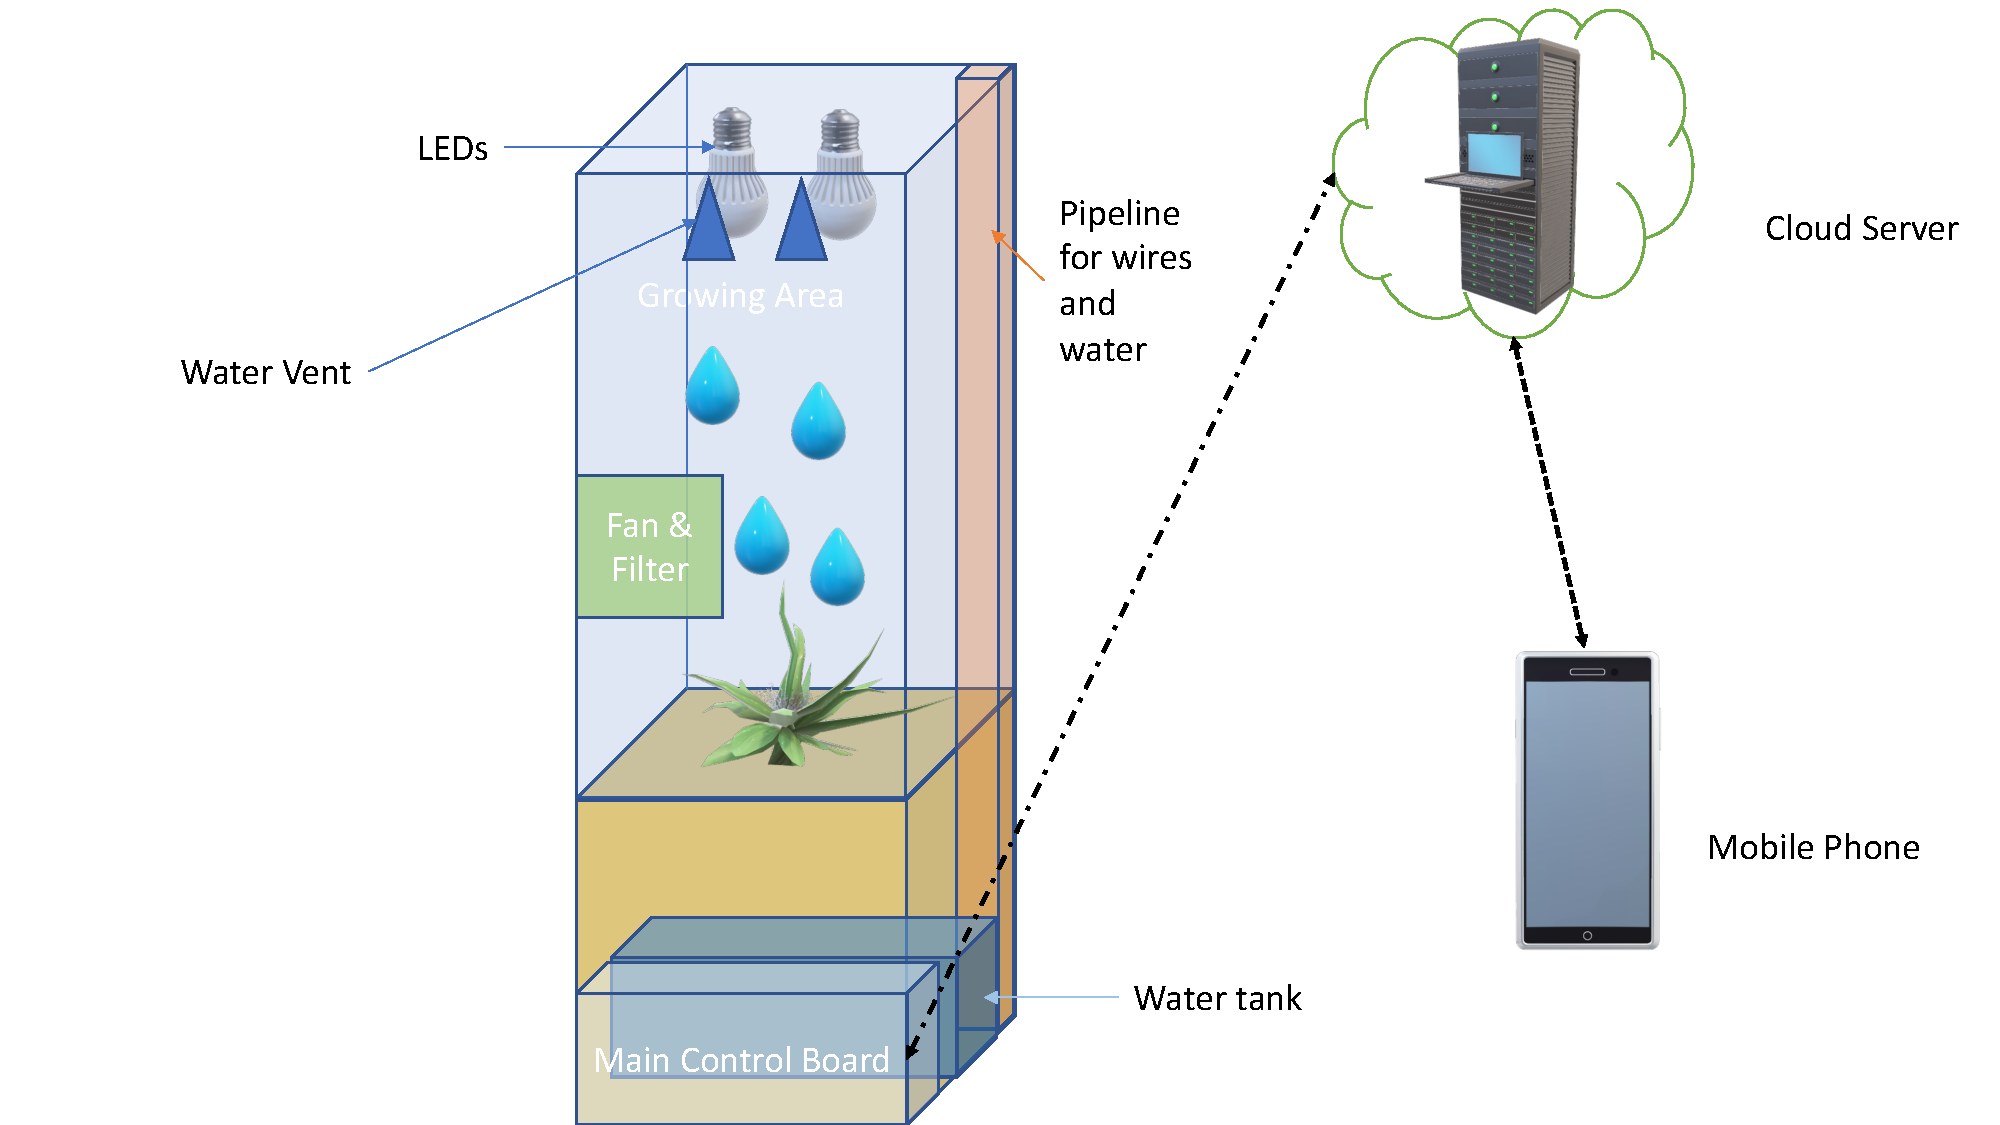
\includegraphics[width=0.8\textwidth]{Figure/visual_overview.pdf}
\caption{Overview of the model}
\label{fig:visual_overview}
\end{figure}

\begin{figure}[!htb]
\centering
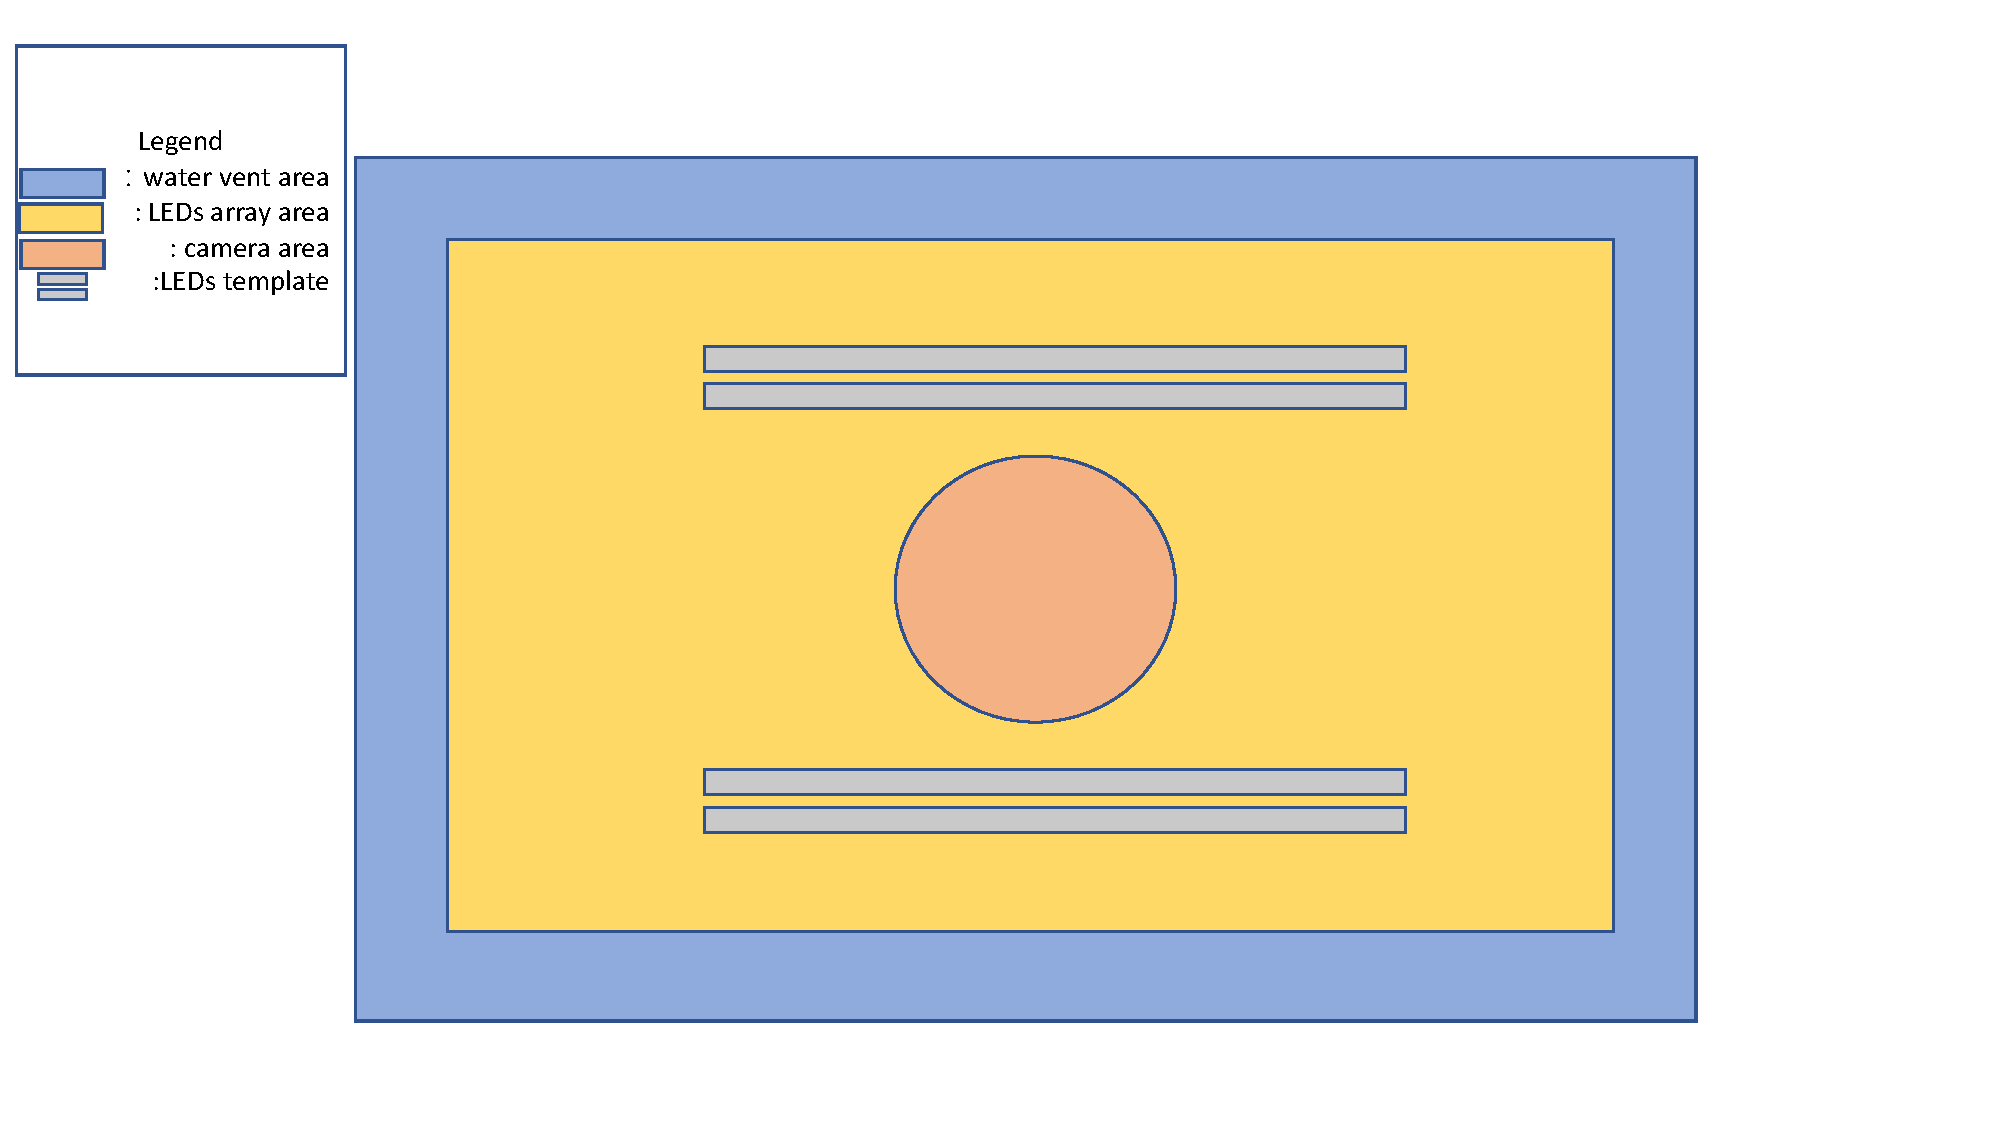
\includegraphics[width=0.8\textwidth]{Figure/upper_level.pdf}
\caption{Model's top platform design}
\label{fig:visual_up}
\end{figure}

\begin{figure}[!htb]
\centering
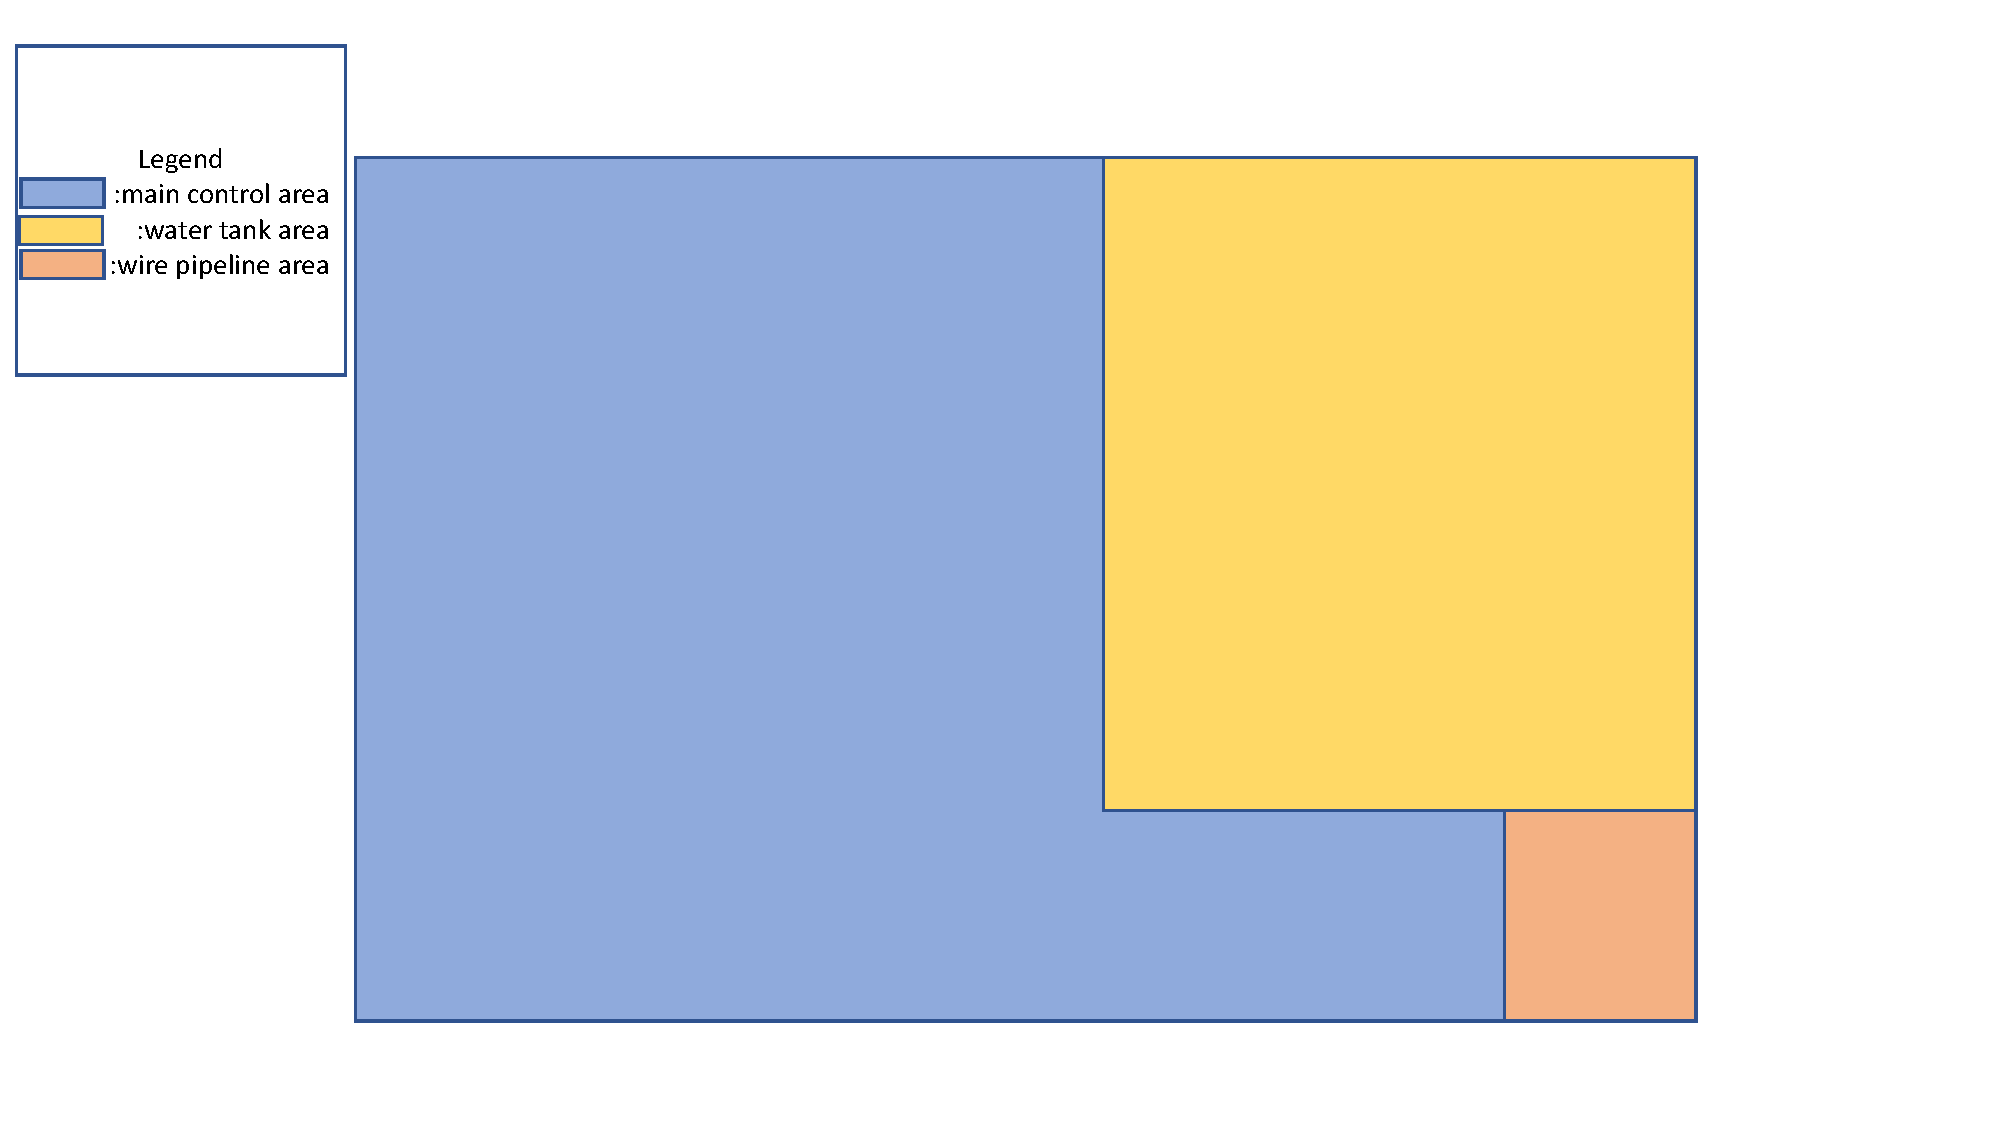
\includegraphics[width=0.8\textwidth]{Figure/lower_level.pdf}
\caption{Model's lower platform design}
\label{fig:visual_low}
\end{figure}

\clearpage

% A pictorial representation of your project that puts your solution in context. Include other external systems relevant to your project (e.g. if your solution connects to a phone via Bluetooth, draw a dotted line between your device and the phone). Note that this is not a block diagram and should explain how the solution is used, not a breakdown of inner components.

\subsection{High-Level Requirement List}
 % A list of three quantitative characteristics that this project must exhibit in order to solve the problem. Each high-level requirement must be stated in complete sentences and displayed as a bulleted list. Avoid mentioning "cost" as a high level requirement.
\begin{enumerate}
    \item There is a main planting cube. The model should be able to hold a fully functional environment-controlling system.
    \item The environment-controlling system includes:
        \begin{enumerate}
        \item Multiple adjustable LEDs to provide demanded light.
        \item A temperature-controlling system that can maintain the temperature.
        \item A humidity-controlling system that can maintain the humidity.
        \end{enumerate}
    \item A filter for the input and out gas, which should filter the harmful particles.
    \item A fan can input and output the air according to the demands.
    \item A camera that can monitor the plants: OV2640/OV5640 (have not determined)
    \item A 5V relay for the water vent.
    \item Several environment detectors should be installed, including:
        \begin{enumerate}
            \item Temperature: DHT22\cite{dht22}
            \item Humidity: DHT22\cite{dht22}
            \item Illumination detector.
            \item Air quality.
        \end{enumerate}
    \item A mobile phone app that can receive the data and adjust the settings.
\end{enumerate}
